\chapter{Deployment}
In questo capitolo verranno illustrate le modalità e gli strumenti utilizzati per effettuare il deploy dell'applicazione sviluppata.

\section{Node-NPM}
La prima modalità utilizzata per effettuare il deploy del servizio è sta quella basata su \emph{Node} ed \emph{npm}. Per poter quindi eseguire questi step sarà necessario installare o verificare l'installazione dei seguenti componenti.
\begin{itemize}
    \item MongoDB
    \item Node
    \item npm
\end{itemize}
Per verificare l'installazione di MongoDB sarà sufficiente lanciare il comando \inlinecode{bash}{mongod -version}, nel caso non fosse presente bisognerà procedere ad installarlo. Analogamente con i comandi \inlinecode{bash}{node -v} e \inlinecode{bash}{npm -v} si verificherà la versione installata degli altri due.

Una volta che l'ambiente è stato correttamente impostato sarà sufficiente utilizzare \emph{git} per importare il progetto, oppure scaricarlo manualmente direttamente dalla pagina web del repository.

\subsection{Local}
Per le fasi di sviluppo il sistema è stato utilizzato in modalità locale, con l'obiettivo di verificarne il funzionamento in itinere. Per fare ciò è stato necessario avviare localmente le due componenti, server e client.

Per avviare il server dopo essersi spostati all'interno dell'omonima cartella con il terminale bisognerà eseguire i seguenti comandi:

\begin{lcverbatim}
    npm install
    set LUPUS_SERVER_PORT=8081
    node server.js
\end{lcverbatim}

Il primo si occuperà di installare tutte le dipendenze necessarie, mentre l'ultimo avvierà effettivamente il server. Per quanto riguarda invece il secondo comando mostrato, il suo utilizzo è opzionale in quanto all'interno del progetto la variabile d'ambiente riportata viene impostata di default al valore \emph{8080}, perciò l'utilizzo del comando si riduce al solo caso in cui sia necessario utilizzare una porta diversa.

Ora per avviare il client bisognerà analogamente da un nuovo terminale spostarsi nella cartella corretta, poi eseguire i seguenti comandi:

\begin{lcverbatim}
    npm install
    set REACT_APP_SERVER_PORT=8081
    npm run build
    serve -s build
\end{lcverbatim}

Dopo aver installato tutte le dipendenze sarà necessario eseguire il secondo comando per modificare la porta alla quale contattare il server solo nel caso si fosse modificata rispetto a quella di default \emph{8080}. I seguenti comandi si occuperanno di creare la build e rendere l'applicazione accessibile online come mostrato nella figura \ref{fig:serve}.

\begin{figure}[H]
\centering
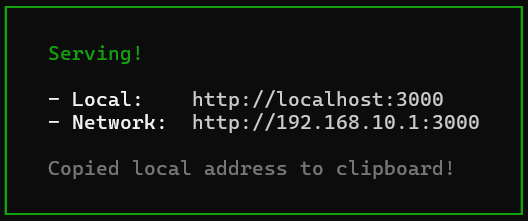
\includegraphics[width=0.7\textwidth]{img/serve.png}
\caption{Output del comando serve}
\label{fig:serve}
\end{figure}

\subsection{Distributed}
Per la fase di test eseguita in maniera distribuita è stato necessario introdurre alcuni strumenti ulteriori. Per raggiungere questo obiettivo sono stati quindi utilizzati anche:
\begin{itemize}
    \item Ngrok\cite{ngrok}
    \item GitHub Pages\cite{gitHubreactghpages}
\end{itemize}

Il primo è un reverse proxy server cross-platform con cui è possibile esporre un server locale, collocato dietro NAT, e firewall alla rete Internet tramite secure tunnel. Dopo aver creato un dominio dalla dashboard messa a disposizione sul loro sito utilizzando il comando  
\begin{lcverbatim}
    ngrok tunnel --label edge=edghts_*** http://localhost:8080
\end{lcverbatim}
sarà possibile connettersi al server sulla macchina locale anche dalla rete esterna all'indirizzo \inlinecode{bash}{wise-resolved-wasp.ngrok-free.app}.

Il codice del client dovrà poi essere modificato per sostituire l'indirizzo \emph{localhost} con quello pubblico. Effettuata la sostituzione è stato sfruttato il servizio offerto da GitHub, ovvero GitHub Pages.

Pages permette di fare hosting di un sito web direttamente dal repository del progetto. Avendo aggiunto anche \inlinecode{bash}{"deploy": "gh-pages -d build"} agli script sarà possibile eseguire il comando
\begin{lcverbatim}
    npm run deploy -- -m "Deploy message"
\end{lcverbatim}
per effettuare la build del client e pushare la nuova versione dell'applicazione.

Dopo aver svolto tutti gli step sarà possibile accedere al sito all'indirizzo
\begin{lcverbatim}
    https://andrea-serafini.github.io/Lupus/
\end{lcverbatim}
per poter utilizzare il sistema collegandosi da remoto al server locale.

\section{Docker}
Per effettuare un deployment semplificato e indipendente dall'architettura della quale si dispone sono stati impostati i file necessari per l'utilizzo di Docker.
Una volta installata e avviata l'applicazione di Docker i comandi da eseguire da linea di comando saranno:
\begin{lcverbatim}
#Per avviare
    docker compose up --build

#Per terminare
    docker compose down
\end{lcverbatim}

La struttura del progetto e dei conseguenti file \emph{docker-compose} permette sia di avviare tutti i container insieme, che di avviare in maniera separata il client e la coppia server-database.